% [原文 p.149]
% 引理 4.13 的陈述起于原书 p.148 末行（归 ch04a），本块自其证明起。
这里不复习收缩核（retract）的定义。论证中只用到收缩核所具有的性质 $H^i(U,\Z_U)\cong H^i(C,\Z_C)$（$\forall i$）。

\begin{proof}
指数序列（exponential sequence）
\[
0\to\Z_U\xrightarrow{\,2\pi\sqrt{-1}\,}\cO_U\xrightarrow{\ \exp\ }\cO_U^*\to 1
\]
在 $\cO_U$ 含幂零元时仍然正合。由其上同调正合列得
\[
0=H^1(U,\cO_U)\to H^1(U,\cO_U^*)\cong\Pic(U)\to H^2(U,\Z_U),
\]
故 (1) 得证。又若 $\mathrm{red}(U)$ 以 $C$ 为收缩核，则 $H^2(U,\Z_U)=H^2(C,\Z_C)=\bigoplus\Z[C_i]$，这正是 (2) 的含义。
\end{proof}

% [Tutor Note: 引理 (2) 的用处是：要判断 $Y$ 上两个线丛是否同构，只需比较它们与例外曲线（以及 $\Delta$ 的分支）的交点数，不必控制整个开集上的整体行为。]

\begin{corollaryp}{4.14}
设 $f\colon Y\to(P\in X)$ 是曲面奇点芽的奇点消解，且 $R^1f_*\cO_Y=0$；$I\subset\cO_{P,X}$ 是极大理想。此时存在有效 Cartier 除子 $E\subset Y$，使 $I\cO_Y=\cO_Y(-E)$，并对一切 $\nu>0$ 有 $I^\nu=f_*\cO_Y(-\nu E)$。
\end{corollaryp}

\begin{proof}
取 $\cO_Y(-E)$ 为 $I\cO_Y$ 的除子部分。此时 $\cO_Y(-E)\supset I\cO_Y$，且 $\Sigma:=\Supp\bigl(\cO_Y(-E)/I\cO_Y\bigr)$ 是有限集。因此 $f^*I\to\cO_Y(-E)$ 在 $Y\setminus\Sigma$ 上是满射，故 $\cO_Y(-E)$ 是 $f$-nef 的。由引理 4.13，$\cO_Y(-E)$ 是 $f$-自由的。由 $E\ne\varnothing$ 得 $I\subseteq f_*\cO_Y(-E)\subseteq\cO_X$，故 $I\cO_Y\subset\cO_Y(-E)$。由于 $I$ 是极大理想，有 $f_*\cO_Y(-E)=I$；再由 $\cO_Y(-E)$ 的 $f$-自由性得到 $I\cO_Y=\cO_Y(-E)$。

下面用关于 $\nu$ 的归纳法证明 $f_*\cO_Y(-\nu E)=I^\nu$ 与 $R^1f_*\cO_Y(-\nu E)=0$（$\forall\nu>0$）。取一般元 $\alpha,\beta\in I$，使 $\cO_Y(-E)$ 的全局截面 $f^*\alpha,f^*\beta$ 满足
\[
(f^*\alpha=0)\cap(f^*\beta=0)=\varnothing .
\]
此时 $\varphi:=(f^*\alpha,f^*\beta)\colon\cO_Y^{\oplus2}\to\cO_Y(-E)$ 是满射，且由行列式计算得到完全序列
\[
0\to\cO_Y(E)\to\cO_Y^{\oplus2}\xrightarrow{\ \varphi\ }\cO_Y(-E)\to 0 .
\]

% [原文 p.150]
由此得到下列完全序列
\[
F_\nu\colon\quad 0\to\cO_Y(-(\nu-1)E)\to\cO_Y(-\nu E)^{\oplus2}\to\cO_Y(-(\nu+1)E)\to 0 .
\]
由 $F_0$ 得到满射 $R^1f_*\cO_Y^{\oplus2}\twoheadrightarrow R^1f_*\cO_Y(-E)$，故 $\nu=1$ 的结论成立。设 $k\ge 1$。若关于 $\nu\le k$ 的结论成立，则由 $F_k$ 得 $f_*\cO_Y(-(k+1)E)=(\alpha,\beta)I^k$，且 $R^1f_*\cO_Y(-(k+1)E)=0$。又 $f_*\cO_Y(-(k+1)E)\supseteq I^{k+1}$，故 $\nu=k+1$ 的结论成立。
\end{proof}

\begin{theoremp}{4.15}
有一个成立。其中 $\Delta_j$ 用 $\bullet$ 号表示，$m$ 为例外曲线的条数。
\begin{enumerate}[label=(\arabic*),leftmargin=*]
\item $\lfloor\Delta\rfloor$ 有 2 个解析分支且 $\Delta=\lfloor\Delta\rfloor$，$m\ge 0$，并且 $\Gamma^*$ 等于
\begin{center}
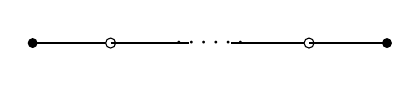
\begin{tikzpicture}[scale=0.9]
\fill (0,0) circle (2pt);
\draw[thin] (0,0)--(1.1,0);
\draw[thin,fill=white] (1.1,0) circle (2pt);
\draw[thin] (1.1,0)--(2.2,0);
\draw[thin] (2.8,0)--(3.9,0);
\draw[thin,fill=white] (3.9,0) circle (2pt);
\draw[thin] (3.9,0)--(5,0);
\fill (5,0) circle (2pt);
\node at (2.5,0) {$\cdots\cdots$};
\end{tikzpicture}
\end{center}
$(X,\Delta)$ 为 dlt 的情形，正是 $X$ 非奇异、$\Delta$ 的 2 个不可约成分横截相交的情形。
\item $\lfloor\Delta\rfloor$ 只有 1 个解析分支且 $\Delta=\lfloor\Delta\rfloor$，$m\ge 3$，并且 $\Gamma^*$ 等于
\begin{center}
\begin{tikzpicture}[scale=0.9]
\fill (0,0) circle (2pt);
\draw[thin] (0,0)--(1.1,0);
\draw[thin,fill=white] (1.1,0) circle (2pt);
\draw[thin] (1.1,0)--(2.2,0);
\draw[thin] (2.8,0)--(3.9,0);
\draw[thin,fill=white] (3.9,0) circle (2pt);
\draw[thin] (3.9,0)--(5.1,0);
\draw[thin,fill=white] (5.1,0) circle (2pt);
\draw[thin] (5.1,0)--(5.1,1.05);
\draw[thin] (5.1,0)--(5.1,-1.05);
\draw[thin,fill=white] (5.1,1.05) circle (2pt);
\draw[thin,fill=white] (5.1,-1.05) circle (2pt);
\node at (5.6,1.05) {$2$};
\node at (5.6,-1.05) {$2$};
\node at (2.5,0) {$\cdots\cdots$};
\end{tikzpicture}
\end{center}
此时 $(X,\Delta)$ 不是 dlt 的。
\item $\lfloor\Delta\rfloor$ 只有一个解析分支，$m\ge 0$，并且 $\Gamma^*$ 等于
\begin{center}
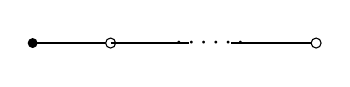
\begin{tikzpicture}[scale=0.9]
\fill (0,0) circle (2pt);
\draw[thin] (0,0)--(1.1,0);
\draw[thin,fill=white] (1.1,0) circle (2pt);
\draw[thin] (1.1,0)--(2.2,0);
\draw[thin] (2.8,0)--(4,0);
\draw[thin,fill=white] (4,0) circle (2pt);
\node at (2.5,0) {$\cdots\cdots$};
\end{tikzpicture}
\end{center}
此时 $(X,\lfloor\Delta\rfloor)$ 是 plt 的。
\end{enumerate}
\end{theoremp}

\begin{proof}
要处理的是定理 4.7(4)–(5) 的情形，故 $\Gamma$ 是树，且至多只有 1 个分叉点。

如记号 4.1 中那样令 $A=\sum a_iE_i$。定理 4.7 中已经看到，对每个 $i$ 都能找到线性组合 $B=\sum b_iE_i$，使 $(B\cdot E_i)\le(A\cdot E_i)$。（但在 (3) 的情形要反过来，用满足 $(B\cdot E_i)\ge(A\cdot E_i)$ 的 $B$。）
\begin{enumerate}[label=(\arabic*),leftmargin=*]
\item 假设 $\lfloor\Delta\rfloor$ 有 2 个解析分支。此时存在如下子图。
\begin{center}
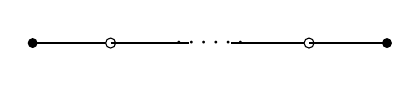
\begin{tikzpicture}[scale=0.9]
\fill (0,0) circle (2pt);
\draw[thin] (0,0)--(1.1,0);
\draw[thin,fill=white] (1.1,0) circle (2pt);
\draw[thin] (1.1,0)--(2.2,0);
\draw[thin] (2.8,0)--(3.9,0);
\draw[thin,fill=white] (3.9,0) circle (2pt);
\draw[thin] (3.9,0)--(5,0);
\fill (5,0) circle (2pt);
\node at (2.5,0) {$\cdots\cdots$};
\end{tikzpicture}
\end{center}
设 $E_1,\dots,E_n$（$n\ge 1$）是标 $\circ$ 的曲线，令 $B=-E_1-\cdots-E_n$，便得到 (1)。
\item 设 $\lfloor\Delta\rfloor$ 只有 1 个解析分支，且 $\Gamma^*$ 有 1 个分叉点。此时存在如下子图。
\begin{center}
\begin{tikzpicture}[scale=0.9]
\fill (0,0) circle (2pt);
\draw[thin] (0,0)--(1.1,0);
\draw[thin,fill=white] (1.1,0) circle (2pt);
\draw[thin] (1.1,0)--(2.2,0);
\draw[thin] (2.8,0)--(3.9,0);
\draw[thin,fill=white] (3.9,0) circle (2pt);
\draw[thin] (3.9,0)--(5.1,0);
\draw[thin,fill=white] (5.1,0) circle (2pt);
\draw[thin] (5.1,0)--(5.1,0.94);
\draw[thin] (5.1,0)--(5.1,-0.94);
\draw[thin] (5.1,1.10)--(5.19,1.02)--(5.1,0.94)--(5.01,1.02)--cycle;
\draw[thin] (5.1,-1.10)--(5.19,-1.02)--(5.1,-0.94)--(5.01,-1.02)--cycle;
\node at (2.5,0) {$\cdots\cdots$};
\end{tikzpicture}
\end{center}
令 $B$ 为系数 $-1$ 的 $\circ$ 曲线与系数 $-1/2$ 的 $\diamond$ 曲线组成的线性组合。像定理 4.7(3) 那样计算，便得到 (2)。
\item 剩下的只有 (3) 的情形。令 $E=E_1\cup\cdots\cup E_n$、$B=-(E_1+\cdots+E_n)$。此时对一切 $i$ 有
\[
(B\cdot E_i)\ge\bigl((K_Y+\lfloor f_*^{-1}\Delta\rfloor)\cdot E_i\bigr).
\]
不过对链右端的曲线，上述不等式是严格的。因此由推论 4.2，对一切 $i$ 有 $a_i>-1$，即 $(X,\lfloor\Delta\rfloor)$ 是 plt 的。
\end{enumerate}
\end{proof}

% [Tutor Note: (1) 中 $\Delta$ 的两个分支横截相交时 $X$ 非奇异；一旦两分支相切，dlt 就不再成立。(2) 的图正是定理 4.7(3) 的图形，差别只在两端的叶子现在被 $\Delta$ 的分支取代。]

% [原文 p.151]
\begin{theorem*}{4.16}
设 $(0\in X,\Delta)$ 是对数标准对，$f\colon Y\to X$ 是极小奇点消解，$\Gamma$ 是例外曲线 $E=\bigcup E_i$ 的对偶图。设 $\Gamma$ 只有 1 个分叉点，其枝恰有 3 条，长度分别为 $n_1-1$、$n_2-1$、$n_3-1$。此时
\[
\frac1{n_1}+\frac1{n_2}+\frac1{n_3}\ge 1 .
\]
其中若 $(0\in X,\Delta)$ 是 dlt 的，则不等式严格成立。
\end{theorem*}

遗憾的是，这一结论的逆不成立。曲线的自交点数值必须满足与枝长相应的某种条件。这些内容在许多文献（例如 [K+92] 第 3 章）中有详细论述。

% [原文 p.152]
\begin{proof}
任意选取 $\Gamma$ 的一条枝，它可以表示为下图。
\begin{center}
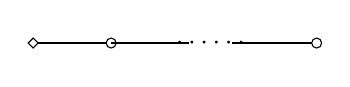
\begin{tikzpicture}[scale=0.9]
\draw[thin] (0,0.07)--(0.07,0)--(0,-0.07)--(-0.07,0)--cycle;
\draw[thin] (0.07,0)--(1.1,0);
\draw[thin,fill=white] (1.1,0) circle (2pt);
\draw[thin] (1.1,0)--(2.2,0);
\draw[thin] (2.8,0)--(4,0);
\draw[thin,fill=white] (4,0) circle (2pt);
\node at (2.5,0) {$\cdots\cdots$};
\end{tikzpicture}
\end{center}
其中 $\diamond$ 表示分叉点，$m$ 表示枝长（顶点 $\circ$ 的个数）。$B$ 通过如下指定分叉点与各枝上的系数来构造。
\begin{center}
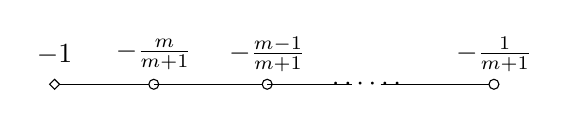
\begin{tikzpicture}[scale=0.9]
\draw[thin] (0,0.07)--(0.07,0)--(0,-0.07)--(-0.07,0)--cycle;
\node at (0,0.42) {$-1$};
\draw[thin] (0.07,0)--(1.4,0);
\draw[thin,fill=white] (1.4,0) circle (2pt);
\node at (1.4,0.42) {$-\frac{m}{m+1}$};
\draw[thin] (1.4,0)--(3.0,0);
\draw[thin,fill=white] (3.0,0) circle (2pt);
\node at (3.0,0.42) {$-\frac{m-1}{m+1}$};
\draw[thin] (3.0,0)--(4.2,0);
\draw[thin] (4.6,0)--(6.2,0);
\draw[thin,fill=white] (6.2,0) circle (2pt);
\node at (6.2,0.42) {$-\frac{1}{m+1}$};
\node at (4.4,0) {$\cdots\cdots$};
\end{tikzpicture}
\end{center}
于是
\[
(B\cdot E_j)
\begin{cases}
=b_j-3+\sum_i 1/n_i, & E_j\ \text{为分叉点的情形},\\
\le b_j-2, & \text{其他情形}.
\end{cases}
\]
故若 $\sum_i1/n_i\le 1$，则 $(B\cdot E_j)\le d_j$。而且若 $\sum_i1/n_i<1$，则至少有一个严格不等式。
\end{proof}

\begin{theoremp}{4.17}
设 $(0\in X)$ 是正规曲面奇点，$f\colon Y\to X$ 是极小奇点消解，$\Gamma$ 是 $f$-例外曲线 $E=\bigcup E_i$ 的对偶图。假设下列条件之一成立。
\begin{enumerate}[label=(\arabic*),leftmargin=*]
\item $\Gamma$ 是链。
\item $\Gamma$ 是只有 1 个分叉点的树，该分叉点恰有 3 条枝。设各枝的长度为 $n_i-1$，则 $\sum_i1/n_i>1$。此外，枝上任何曲线的自交点数值都是 $-2$。
\end{enumerate}
此时 $(0\in X)$ 是 klt 的。
\end{theoremp}

\begin{proof}
(1) 的情形，令 $B=-(E_1+\cdots+E_n)$。此时对每个 $i$ 有 $(B\cdot E_i)\ge d_i$，而且对链两端的曲线成立严格不等式。故由推论 4.2，对每个 $i$ 有 $a_i>-1$。于是 $(0\in X)$ 是 klt 的。
(2) 的情形，像定理 4.16 那样选取 $B$，同样论证即可。
\end{proof}

本书并不需要，但为求完备，下面再给出对数终端曲面奇点的另一个特征刻画。它容易由注 4.21 与命题 5.20 推出。

\begin{proposition}{4.18}
对正规解析曲面的芽 $(0\in X)$，下列条件等价。
\begin{enumerate}[label=(\arabic*),leftmargin=*]
\item $(0\in X)$ 是对数终端的；
% [原文 p.153]
\item $(0\in X)$ 是余维数 1 处自由的群作用给出的 $(0\in\C^2)$ 的商空间；
\item $(0\in X)$ 是有限群作用给出的 $(0\in\C^2)$ 的商空间。
\end{enumerate}
\end{proposition}

\par\medskip\noindent\textbf{4.19}\quad 本节中的证明，除注 4.9、命题 4.10、定理 4.12、命题 4.18 这 4 个例外，在任意特征下都成立。命题 4.10 与定理 4.12 在任意特征下成立，这一点可以用 [Art66] 证明。注 4.9 与命题 4.18 在正特征下，即使对 Du Val 奇点也不成立（参见 [Lip69]）。\hfill$\square$

% [Tutor Note: 4.19 说明本章此前的论证几乎不依赖特征 0，唯一的代价是把 4 个结论排除在外。正特征下的反例 [Lip69] 表明 Du Val 奇点的“标准性”在正特征下会失效。]

\section{Du Val 奇点}
\takeaway{本节把二维标准奇点等同于 Du Val 奇点，给出其方程分类 A、D、E 与极小消解的对偶图。工具是交换爆破下 $K$ 的变换公式与图上加权亏格的计算：$A$-$D$-$E$ 图恰是亏格 0 的负定树。}

本节的目标是用简单而具体的方程描述 Du Val 奇点。

\begin{theorem*}{4.20}
设 $(0\in X)$ 是正规曲面奇点的芽。下列条件等价。
\begin{enumerate}[label=(\arabic*),leftmargin=*]
\item $(0\in X)$ 是标准奇点。
\item $(0\in X)$ 是 Du Val 奇点。
\item $(0\in X)$ 与由下列方程之一定义的特异点解析同构。
\begin{align*}
&\text{A.}\quad x^2+y^2+z^{n+1}=0.\\
&\text{D.}\quad x^2+y^2z+z^{n-1}=0.\\
&\text{E.}\quad x^2+y^3+z^4=0,\quad x^2+y^3+yz^3=0,\quad x^2+y^3+z^5=0.
\end{align*}
\end{enumerate}
\end{theorem*}

\begin{remark}{4.21}
Du Val 奇点在许多不同的情形中自然出现，并且有许多种刻画方法 [Dur79]。这里不加证明地叙述其中两条。
\begin{enumerate}[label=(\arabic*),leftmargin=*]
\item Du Val 奇点正是 $SL(2,\C)$ 的有限子群作用给出的 $\C^2$ 的商空间。
\item Du Val 奇点是单纯奇点（simple singularity）。（即 Du Val 奇点的小形变只产生有限个奇点。）
\end{enumerate}
此外，“是 Du Val 的”这一性质是开条件。即若 $(f=0)$ 是 Du Val 的而 $g$ 任意，则当 $|\eps|\ll 1$ 时 $(f+\eps g=0)$ 是 Du Val 的。分析 4.25 即可看出这一点，但也可由推论 5.24 与定理 5.42 推出。
% [原文 p.154]
这是重要的概念，但以后并不需要。
\end{remark}

\begin{proof}
标准奇点是 Du Val 奇点，这一点已在定理 4.5 中证明。若 $(0\in X)$ 是定理 4.20(3) 所列奇点之一，则具体计算奇点消解，便可证明它是 Du Val 的。这可用下面两个步骤验证。
\begin{enumerate}[label=(\arabic*),leftmargin=*]
\item 若 $(0\in X)$ 是曲面二重点，$p\colon B_0X\to X$ 是原点处的爆破，则
\[
K_{B_0X}=p^*K_X .
\]
\item 若 $(0\in X)$ 是定理 4.20(3) 的奇点之一，则 $B_0X$ 的任何一个奇点也是定理 4.20(3) 中的奇点。
\end{enumerate}
执行这些计算，并确认所得例外曲线的对偶图正是定理 4.22 所描述者，对读者将十分有益。

其次，证明若 $(0\in X)$ 是 Du Val 的，则它是标准奇点。这虽可由定理 3.3 推出，但下面的直接证明更简单。$f\colon Y\to X$ 是极小奇点消解，$E=\bigcup E_i$ 是例外曲线。由定理 4.12，有 $H^1(Y,\cO_Y)=0$。$Y$ 上的两个线丛 $\cO_Y$ 与 $\cO_Y(K_Y)$ 与一切曲线 $E_i$ 的交点数均为 $0$。故由引理 4.13，$\cO_Y\cong\cO_Y(K_Y)$。特别地，$\cO_Y(K_Y)$ 由一个整体截面 $\sigma\in H^0(Y,\cO_Y(K_Y))$ 生成。于是 $f_*\cO_Y(K_Y)$ 由单个元 $f_*\sigma$ 生成，从而是局部自由的。存在自然定义的映射
\[
f_*\cO_Y(K_Y)\to\cO_X(K_X),
\]
它在 $0$ 之外是同构。由于 $f_*\cO_Y(K_Y)$ 局部自由，这意味着 $f_*\cO_Y(K_Y)=\cO_X(K_X)$。因此 $K_X$ 是 Cartier 的，且 $f^*\cO_X(K_X)=\cO_Y(K_Y)$ 成立。这说明 $(0\in X)$ 是标准奇点。

剩下要证的部分是下述更精确结果的特殊情形。
\end{proof}

% [原文 p.155]
\begin{theoremp}{4.22}
Du Val 奇点的嵌入维数（embedding dimension），即把 $m$ 取为极大理想时 $m/m^2$ 作为向量空间的维数，总是 $3$。适当选取局部解析坐标后，下述列表给出 Du Val 奇点的完整清单。其中例外曲线都是 $(-2)$-曲线（即满足 $(C^2)=-2$ 的非奇异有理曲线 $C$）。
\begin{enumerate}[label={},leftmargin=*]
\item[A.] 奇点 $A_n$（$n\ge 1$）的方程为 $x^2+y^2+z^{n+1}=0$，对偶图由 $n$ 个顶点组成，如下图所示。
\begin{center}
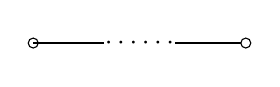
\begin{tikzpicture}[scale=0.9]
\draw[thin,fill=white] (0,0) circle (2pt);
\draw[thin] (0,0)--(1.0,0);
\node at (1.5,0) {$\cdots\cdots$};
\draw[thin] (2.0,0)--(3.0,0);
\draw[thin,fill=white] (3.0,0) circle (2pt);
\end{tikzpicture}
\end{center}
\item[D.] 奇点 $D_n$（$n\ge 4$）的方程为 $x^2+y^2z+z^{n-1}=0$，对偶图由 $n$ 个顶点组成，如下图所示。
\begin{center}
\begin{tikzpicture}[scale=0.9]
\draw[thin,fill=white] (0,0) circle (2pt);
\draw[thin] (0,0)--(1.0,0);
\node at (1.5,0) {$\cdots\cdots$};
\draw[thin] (2.0,0)--(2.6,0);
\draw[thin,fill=white] (2.6,0) circle (2pt);
\draw[thin] (2.6,0)--(2.6,0.95);
\draw[thin,fill=white] (2.6,0.95) circle (2pt);
\draw[thin] (2.6,0)--(3.6,0);
\draw[thin,fill=white] (3.6,0) circle (2pt);
\draw[thin] (3.6,0)--(4.6,0);
\draw[thin,fill=white] (4.6,0) circle (2pt);
\end{tikzpicture}
\end{center}
\item[E.] 奇点 $E_6$（或 $E_7$，$E_8$）的方程为 $x^2+y^3+z^4=0$（或 $x^2+y^3+yz^3=0$，$x^2+y^3+z^5=0$），对偶图由 $6$（或 $7$，$8$）个顶点组成，如下图所示。
\begin{center}
\begin{tikzpicture}[scale=0.9]
\draw[thin,fill=white] (0,0) circle (2pt);
\draw[thin] (0,0)--(1.0,0);
\node at (1.5,0) {$\cdots\cdots$};
\draw[thin] (2.0,0)--(2.6,0);
\draw[thin,fill=white] (2.6,0) circle (2pt);
\draw[thin] (2.6,0)--(2.6,0.95);
\draw[thin,fill=white] (2.6,0.95) circle (2pt);
\draw[thin] (2.6,0)--(3.6,0);
\draw[thin,fill=white] (3.6,0) circle (2pt);
\draw[thin] (3.6,0)--(4.6,0);
\draw[thin,fill=white] (4.6,0) circle (2pt);
\end{tikzpicture}
\end{center}
\end{enumerate}
反之，设 $Y$ 是非奇异曲面，$E\subset Y$ 是使对偶图为上述图之一的固有曲线的集合。此时 $E\subset Y$ 是某曲面 $0\in X$ 的极小奇点消解，其中 $0$ 对应 Du Val 奇点。
\end{theoremp}

\begin{proof}
设 $(0\in X)$ 是 Du Val 奇点，$f\colon Y\to X$ 是其极小奇点消解。$E=\bigcup E_i$ 是例外曲线，$\Gamma$ 是其对偶图。首先证明 $\Gamma$ 是上述图之一。

由 $(0\in X)$ 是 lc 的。由定理 4.7，$\Gamma$ 或是链（$A$-型），或满足下述条件：$\Gamma$ 恰有 $1$ 个分叉点，该分叉点有 $3$ 条枝。设各枝的长度为 $n_i-1$，则成立
\[
\frac1{n_1}+\frac1{n_2}+\frac1{n_3}>1 .
\]
满足此条件的正整数组的集合只有 $(2,2,m)$（$D$-型）、$(2,3,3)$、$(2,3,4)$、
% [原文 p.156]
$(2,3,5)$（$E$-型）。故 $\Gamma$ 是上述图之一。

此外，实际计算极小奇点消解即可知，与方程对应的对偶图正是上述各图。

分两个阶段求方程。首先确定曲面 $(0\in X)$ 的超曲面截断，得到某种形式的方程。再利用 $(0\in X)$ 是标准奇点这一事实，在坐标变换下逐步限定方程，最后化为标准形。
\end{proof}

\begin{lemmap}{4.23}
设 $(0\in X)$ 是 Du Val 奇点。此时 $(0\in X)$ 是嵌入维数为 $3$ 的二重点。
\end{lemmap}

\begin{proof}
设 $f\colon Y\to X$ 是极小奇点消解。我们来明确写出成为 $0\in X$ 的超曲面截断的拉回的除子 $Z+\bar C$。

在下面的图中，$\bullet$ 表示 $\bar C$ 的不可约成分，添在 $\circ$ 旁的数表示 $Z$ 中该曲线的重数。$\bar C$ 的取法不唯一。设 $\bar C_1$ 与 $\bar C_2$ 是作为 $\bar C$ 选出的两条曲线，且互不相交。
\begin{center}
\begin{tikzpicture}[scale=0.95]
% A_n
\node at (-1.2,0) {$A_n$:};
\fill (0,0) circle (2pt);
\draw[thin] (0,0)--(1.2,0);
\draw[thin,fill=white] (1.2,0) circle (2pt);
\node at (1.2,0.45) {$1$};
\draw[thin] (1.2,0)--(2.0,0);
\node at (2.5,0) {$\cdots\cdots$};
\draw[thin] (3.0,0)--(3.8,0);
\draw[thin,fill=white] (3.8,0) circle (2pt);
\node at (3.8,0.45) {$1$};
\draw[thin] (3.8,0)--(5.0,0);
\fill (5.0,0) circle (2pt);
% D_n
\node at (-1.2,-1.9) {$D_n$:};
\draw[thin,fill=white] (0,-1.9) circle (2pt);
\node at (0,-1.45) {$1$};
\draw[thin] (0,-1.9)--(1.2,-1.9);
\draw[thin,fill=white] (1.2,-1.9) circle (2pt);
\node at (1.2,-1.45) {$2$};
\draw[thin] (1.2,-1.9)--(2.0,-1.9);
\node at (2.5,-1.9) {$\cdots\cdots$};
\draw[thin] (3.0,-1.9)--(3.8,-1.9);
\draw[thin,fill=white] (3.8,-1.9) circle (2pt);
\node at (3.8,-1.45) {$2$};
\draw[thin] (3.8,-1.9)--(5.0,-1.9);
\draw[thin,fill=white] (5.0,-1.9) circle (2pt);
\node at (5.0,-1.45) {$1$};
\draw[thin] (1.2,-1.9)--(1.2,-2.75);
\draw[thin,fill=white] (1.2,-2.75) circle (2pt);
\node at (1.2,-3.2) {$1$};
\draw[thin] (3.8,-1.9)--(3.8,-2.75);
\fill (3.8,-2.75) circle (2pt);
% E_6
\node at (-1.2,-4.4) {$E_6$:};
\draw[thin,fill=white] (0,-4.4) circle (2pt);
\node at (0,-3.95) {$1$};
\draw[thin] (0,-4.4)--(1.2,-4.4);
\draw[thin,fill=white] (1.2,-4.4) circle (2pt);
\node at (1.2,-3.95) {$2$};
\draw[thin] (1.2,-4.4)--(2.4,-4.4);
\draw[thin,fill=white] (2.4,-4.4) circle (2pt);
\node at (2.4,-3.95) {$3$};
\draw[thin] (2.4,-4.4)--(3.6,-4.4);
\draw[thin,fill=white] (3.6,-4.4) circle (2pt);
\node at (3.6,-3.95) {$2$};
\draw[thin] (3.6,-4.4)--(4.8,-4.4);
\draw[thin,fill=white] (4.8,-4.4) circle (2pt);
\node at (4.8,-3.95) {$1$};
\draw[thin] (2.4,-4.4)--(2.4,-5.25);
\draw[thin,fill=white] (2.4,-5.25) circle (2pt);
\node at (2.4,-5.7) {$2$};
\draw[thin] (2.4,-5.25)--(3.6,-5.25);
\fill (3.6,-5.25) circle (2pt);
% E_7
\node at (-1.2,-7.0) {$E_7$:};
\fill (0,-7.0) circle (2pt);
\draw[thin] (0,-7.0)--(1.2,-7.0);
\draw[thin,fill=white] (1.2,-7.0) circle (2pt);
\node at (1.2,-6.55) {$2$};
\draw[thin] (1.2,-7.0)--(2.4,-7.0);
\draw[thin,fill=white] (2.4,-7.0) circle (2pt);
\node at (2.4,-6.55) {$3$};
\draw[thin] (2.4,-7.0)--(3.6,-7.0);
\draw[thin,fill=white] (3.6,-7.0) circle (2pt);
\node at (3.6,-6.55) {$4$};
\draw[thin] (3.6,-7.0)--(4.8,-7.0);
\draw[thin,fill=white] (4.8,-7.0) circle (2pt);
\node at (4.8,-6.55) {$3$};
\draw[thin] (4.8,-7.0)--(6.0,-7.0);
\draw[thin,fill=white] (6.0,-7.0) circle (2pt);
\node at (6.0,-6.55) {$2$};
\draw[thin] (6.0,-7.0)--(7.2,-7.0);
\draw[thin,fill=white] (7.2,-7.0) circle (2pt);
\node at (7.2,-6.55) {$1$};
\draw[thin] (3.6,-7.0)--(3.6,-7.85);
\draw[thin,fill=white] (3.6,-7.85) circle (2pt);
\node at (3.6,-8.3) {$2$};
% E_8
\node at (-1.2,-9.6) {$E_8$:};
\draw[thin,fill=white] (0,-9.6) circle (2pt);
\node at (0,-9.15) {$2$};
\draw[thin] (0,-9.6)--(1.2,-9.6);
\draw[thin,fill=white] (1.2,-9.6) circle (2pt);
\node at (1.2,-9.15) {$4$};
\draw[thin] (1.2,-9.6)--(2.4,-9.6);
\draw[thin,fill=white] (2.4,-9.6) circle (2pt);
\node at (2.4,-9.15) {$6$};
\draw[thin] (2.4,-9.6)--(3.6,-9.6);
\draw[thin,fill=white] (3.6,-9.6) circle (2pt);
\node at (3.6,-9.15) {$5$};
\draw[thin] (3.6,-9.6)--(4.8,-9.6);
\draw[thin,fill=white] (4.8,-9.6) circle (2pt);
\node at (4.8,-9.15) {$4$};
\draw[thin] (4.8,-9.6)--(6.0,-9.6);
\draw[thin,fill=white] (6.0,-9.6) circle (2pt);
\node at (6.0,-9.15) {$3$};
\draw[thin] (6.0,-9.6)--(7.2,-9.6);
\draw[thin,fill=white] (7.2,-9.6) circle (2pt);
\node at (7.2,-9.15) {$2$};
\draw[thin] (7.2,-9.6)--(8.4,-9.6);
\fill (8.4,-9.6) circle (2pt);
\draw[thin] (2.4,-9.6)--(2.4,-10.45);
\draw[thin,fill=white] (2.4,-10.45) circle (2pt);
\node at (2.4,-10.9) {$3$};
\end{tikzpicture}
\end{center}
各情形都可验证 $(Z+\bar C_i)\cdot E_j=0$（$\forall j$）与 $(Z\cdot\bar C_i)=2$。故由引理 4.13，$\cO_Y(-Z-\bar C_i)\cong\cO_Y$。于是，由截面
\[
1\in H^0(Y,\cO_Y)\cong H^0(Y,\cO_Y(-Z-\bar C_i))\subset H^0(Y,\cO_Y)=H^0(X,\cO_X)
\]
% [原文 p.157]
所确定的 $X$ 上的函数记为 $g_i$，则 $0\in X$ 的超曲面截断 $C_i=(g_i=0)$ 满足 $f^*C_i=Z+\bar C_i$。

这两个超曲面截断的局部交点 $(C_1\cdot C_2)_X$ 是 $X$ 在 $0$ 处的重数的倍数，而由投影公式可如下计算。
\[
(C_1\cdot C_2)_X=(Z+\bar C_1\cdot\bar C_2)_Y=(Z\cdot\bar C_2)_Y=2 .
\]
于是 $C_i$ 是重数 $2$（或 $1$）的约化曲线奇点，并且是平面奇点。因此 $X$ 的嵌入维数是 $3$（或 $2$）。
\end{proof}

% [Tutor Note: 图里给 A、D、E 型配的重数正是 $Z$ 在极小消解上的系数；两端 $\bullet$ 代表 $\Delta$ 的分支拉回后的曲线。读者可把 $A_n$ 的情形与 $A_n$ 的连分数解消对照，检验这些重数。]

\begin{proof}[定理 4.22 的证明（续）]
\par\medskip\noindent\textbf{注意}\quad 这一结果是引理 5.30 的二维版本。用一般原理的另一个证明如下。$(0\in X)$ 是标准曲面奇点，$0\in C\subset X$ 是一般超曲面截断，$\pi\colon\bar C\to C$ 是正规化。由引理 5.30，$\pi_*\omega_{\bar C}\supset m_{0,C}\omega_C$ 成立。这（用某种局部对偶理论）等价于 $m_{0,C}\cO_C\subset\cO_C$。后者意味着 $C$ 是通常结点或尖点。

于是可知，$(0\in X)$ 在 $\C^3$ 内由 $F=x^2+f(y,z)$ 形式的方程定义。除去解析局部坐标变换后的分类已在 [AGZV85] 中研究，用其方法即可完成定理 4.22 的证明。下面介绍的是把该方法稍加简化的版本。

\par\medskip\noindent\textbf{4.24}\quad 这里反复使用 $4$ 种方法。
\begin{enumerate}[label=(\arabic*),leftmargin=*]
\item Weierstrass 预备定理（Weierstrass preparation theorem）。
\item 若 $a_n$ 是单位（unit）（即存在环元 $v$ 使 $a_n\cdot v=1$），则可由坐标变换 $y\mapsto y-a_{n-1}/na_n$，从多项式 $a_ny^n+a_{n-1}y^{n-1}+\cdots$ 中消去 $y^{n-1}$ 项。
\item 如下形式的 Hensel 引理（Hensel's lemma）。$f(y,z)$ 是幂级数，$f_d(y,z)$ 是给出其首项的 $d$ 次齐次部分。设 $f_d=gh$，且 $g$ 与 $h$ 没有公共因子。此时 $f=GH$ 成立，其中 $G$（或 $H$）是首项等于 $g$（或 $h$）的幂级数。
\item 设 $M_1,M_2,M_3$ 是变量 $x,y,z$ 的单项式，且乘法上互相独立。此时
% [原文 p.158]
形如 $M_1\cdot(\text{单位})+M_2\cdot(\text{单位})+M_3\cdot(\text{单位})$ 的任意幂级数，都可通过适当的坐标变换 $x\mapsto x\cdot(\text{单位})$、$y\mapsto y\cdot(\text{单位})$、$z\mapsto z\cdot(\text{单位})$ 化为 $M_1+M_2+M_3$。
\end{enumerate}

以下 $f_d$ 表示幂级数 $f$ 的 $d$ 次齐次部分。

\par\medskip\noindent\textbf{4.25}\quad 证明分若干阶段进行，依次把方程归结为更简单的形式。

\noindent\textbf{阶段 1}\quad 若 $\mult_0F=1$，则得到非奇异点。以下设 $\mult_0F=2$。

\noindent\textbf{阶段 2}\quad 对 $x^2$ 应用 4.24(1) 与 4.24(2)，把方程归结为
\[
F=(\text{单位})\cdot\bigl(x^2+f(y,z)\bigr)
\]
的形式。

\noindent\textbf{阶段 3}\quad 若 $\mult_0f\le 2$，则对 $f$ 应用 4.24(1)、(2)，得到方程
\[
F=(\text{单位})\cdot\bigl(x^2+(\text{单位})\cdot(y^2+z^m\cdot(\text{单位}))\bigr)\qquad(m\ge 2).
\]
由 4.24(4) 得到 $F=x^2+y^2+z^m$，这些是 $A$-型。

下面设 $\mult_0f=3$，即 $f_3\ne 0$。

\noindent\textbf{阶段 4}\quad 设 $f_3$ 不是一次式的三次方。此时 $f_3=lq$，其中 $l$ 是齐次一次式，且不是 $q$ 的因子。由 4.24(3) 得 $f=LQ$。这里选取坐标，使 $L$ 成为坐标之一 $z$。于是 $f=z(ay^2+\cdots)$；又因 $l$ 不是 $q$ 的因子，有 $a\ne 0$。对 $y^2$ 应用 4.24(1)、(2)，得到形如
\[
(\text{单位})\cdot\bigl(x^2+(\text{单位})\cdot z(y^2+z^m\cdot(\text{单位}))\bigr)\qquad(m\ge 2)
\]
的方程。由 4.24(4)，方程变形为
\[
x^2+z(y^2+z^m)\qquad(m\ge 2),
\]
这就得到 $D$-型。

\noindent\textbf{阶段 5}\quad 剩下的是 $f_3$ 为三次方的情形。4.24(1)、(2) 给出
\[
f=y^3\cdot u+yz^a\cdot u_a+z^b\cdot u_b ,
\]
其中 $a\ge 3$，$b\ge 4$，$u$ 是单位，$u_a,u_b$ 是单位或 $0$。

\noindent\textbf{阶段 6}\quad 设 $u=u(y,z)$ 是单位。此时奇点
\[
X:=\bigl(x^2+y^3\cdot u+yz^a\cdot u_a+z^b\cdot u_b=0\bigr)
\]
为 Du Val 的充要条件是 $a\le 3$ 且 $u_a(0)\ne 0$，或者 $b\le 5$ 且 $u_b(0)\ne 0$。
\end{proof}

% [块边界：原书 p.159（页图 p170）以该充要条件的 [証明] 开始，归 ch04c；本块止于 p.158，定理 4.22 的证明在 ch04c 中以 [证明（续）] 接续。]
